\documentclass[dvisvgm,tikz]{standalone}
\usepackage{circuitikz}
\begin{document}
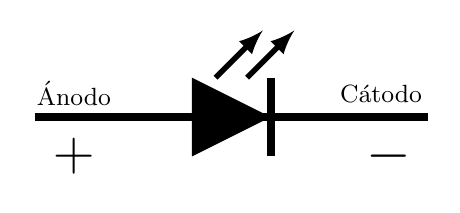
\begin{tikzpicture}
  \draw[line width=1mm] (0.5,1.5) -- (5.5,1.5);
  \draw[line width=1mm] (3.5,1.0) -- (3.5,2.0);
  \fill (2.5,1.0) -- (2.5,2.0) -- (3.5,1.5) -- cycle;
  \node at (1,1.8) {\small Ánodo};
  \node at (4.9,1.8) {\small Cátodo};
  \node at (1,1) {\huge\textbf{$+$}};
  \node at (5,1) {\huge\textbf{$-$}};
  
  \draw[->, line width=2, >=latex] (2.8,2) -- (3.4,2.6);
  \draw[->, line width=2, >=latex] (3.2,2) -- (3.8,2.6);
\end{tikzpicture}
\end{document}